%%%%%%%%%%%%%%%%%%%%%%%%%%%%%%%%%%%%%%%%%
% University Assignment Title Page
% LaTeX Template
% Version 1.0 (27/12/12)
%
% This template has been downloaded from:
% http://www.LaTeXTemplates.com
%
% Original author:
% WikiBooks (http://en.wikibooks.org/wiki/LaTeX/Title_Creation)
%
% License:
% CC BY-NC-SA 3.0 (http://creativecommons.org/licenses/by-nc-sa/3.0/)
%
% Instructions for using this template:
% This title page is capable of being compiled as is. This is not useful for
% including it in another document. To do this, you have two options:
%
% 1) Copy/paste everything between \begin{document} and \end{document}
% starting at \begin{titlepage} and paste this into another LaTeX file where you
% want your title page.
% OR
% 2) Remove everything outside the \begin{titlepage} and \end{titlepage} and
% move this file to the same directory as the LaTeX file you wish to add it to.
% Then add \input{./title_page_1.tex} to your LaTeX file where you want your
% title page.
%
%%%%%%%%%%%%%%%%%%%%%%%%%%%%%%%%%%%%%%%%%

%----------------------------------------------------------------------------------------
%	PACKAGES AND OTHER DOCUMENT CONFIGURATIONS
%----------------------------------------------------------------------------------------

%Fixes pandoc tightlist error
\providecommand{\tightlist}{%
  \setlength{\itemsep}{0pt}\setlength{\parskip}{0pt}}

\documentclass[12pt]{article}
%\renewcommand{\familydefault}{\sfdefault}
\usepackage{amsfonts}
\usepackage{amssymb}
\usepackage{multicol}
\usepackage{graphicx}
\usepackage{titlesec}
\usepackage{longtable}
\usepackage{supertabular}

\usepackage{booktabs}
\setlength{\parindent}{0pt}
\setlength{\parskip}{1em}

\usepackage{hyperref}

%References
\usepackage[
backend=bibtex,
style=numeric,
autocite=footnote,
citestyle=authoryear 
]{biblatex}
\addbibresource{references.bib}
\usepackage[british]{babel}
\usepackage{csquotes}

\usepackage{url}

\usepackage{microtype}


%	Below are optional commands to adjust the document.
%----------------------------------------------------------------------------------------
%----------------------------------------------------------------------------------------
%	Show's overfilled areas.
%----------------------------------------------------------------------------------------
%\overfullrule=2cm
%----------------------------------------------------------------------------------------

%----------------------------------------------------------------------------------------
%	Stop hyphenation.
%----------------------------------------------------------------------------------------
%\widowpenalty=10000
%\clubpenalty=10000
%----------------------------------------------------------------------------------------

%----------------------------------------------------------------------------------------
%	Adds a clear page after each section to start the next on a new page.
%----------------------------------------------------------------------------------------
%\newcommand\sectionbreak{\clearpage}
%----------------------------------------------------------------------------------------

%----------------------------------------------------------------------------------------
%	The following removes section numbering
%----------------------------------------------------------------------------------------
%\renewcommand{\thesection}{}
%\renewcommand{\thesubsection}{\arabic{section}.\arabic{subsection}}
%\makeatletter
%\def\@seccntformat#1{\csname #1ignore\expandafter\endcsname\csname the#1\endcsname\quad}
%\let\sectionignore\@gobbletwo
%\let\latex@numberline\numberline
%\def\numberline#1{\if\relax#1\relax\else\latex@numberline{#1}\fi}
%\makeatother
%----------------------------------------------------------------------------------------

\begin{document}

\begin{titlepage}

\newcommand{\HRule}{\rule{\linewidth}{0.5mm}} % Defines a new command for the horizontal lines, change thickness here

\center % Center everything on the page

%----------------------------------------------------------------------------------------
%	HEADING SECTIONS
%----------------------------------------------------------------------------------------

\textsc{\LARGE University of Brighton}\\[1.5cm] % Name of your university/college
\textsc{\Large Computer Science (Games)}\\[0.5cm] % Major heading such as course name
\textsc{\large Individual Project - CI301}\\[0.5cm] % Minor heading such as course title

%----------------------------------------------------------------------------------------
%	TITLE SECTION
%----------------------------------------------------------------------------------------

\HRule \\[0.4cm]
{ \huge \bfseries Interim Planning and Investigation Report}\\[0.4cm] % Title of your document
\HRule \\[1.5cm]

%----------------------------------------------------------------------------------------
%	AUTHOR SECTION
%----------------------------------------------------------------------------------------

\begin{minipage}{0.4\textwidth}
\begin{flushleft} \large
\emph{Author:}\\
Adam \textsc{Worley} % Your name
\end{flushleft}
\end{minipage}
~
\begin{minipage}{0.4\textwidth}
\begin{flushright} \large
\emph{Supervisor:} \\
Marcus \textsc{Winter} % Supervisor's Name (Manos)
\end{flushright}
\end{minipage}\\[3cm]

% If you don't want a supervisor, uncomment the two lines below and remove the section above
%\Large \emph{Author:}\\
%John \textsc{Smith}\\[2cm] % Your name

%----------------------------------------------------------------------------------------
%	DATE SECTION
%----------------------------------------------------------------------------------------

{\large Hand in Date : 30\textsuperscript{th} of November 2016}\\[2cm] % Date, change the \today to a set date if you want to be precise

%----------------------------------------------------------------------------------------
%	LOGO SECTION
%----------------------------------------------------------------------------------------


\includegraphics[scale=0.60]{Images/BrightonLogo.jpg}\\[1cm] % Include a department/university logo - this will require the graphicx package

%\cite{brightonlogo}


%----------------------------------------------------------------------------------------

\vfill % Fill the rest of the page with whitespace

\end{titlepage}
\tableofcontents
\pagebreak

\section{Project Scope}\label{project-scope}

\subsection{Aims and objectives}\label{aims-and-objectives}

What I will be developing over the upcoming months is an app to help
users get out of bed easier in the morning in a useful and information
rich way.

My aims are:

\begin{itemize}
\tightlist
\item
  Produce an alarm app with all the functionality users are used to.
\item
  Integrate Smartbulb functionality into the app to turn the light on in
  the morning with the alarm.
\item
  To turn off the lights at night without having to get out of bed.
\item
  Provide weather information for the day.
\item
  Inform the user of their schedule for the day and upcoming events.
\item
  Publish the application to the play store for download and use by
  others.
\end{itemize}

\subsection{Stakeholders}\label{stakeholders}

I do not have a client that I am developing my application for and so do
not have a pre-defined user base or stakeholders however, I have
identified the following stakeholders:

\begin{itemize}
\item
  Myself - Not only am I developing the application making me a
  stakeholder, I am also very interested in home automation and waking
  up happy.
\item
  My supervisor, Marcus Winter - By accepting to be my supervisor Marcus
  is also a stakeholder for my application, he will be providing
  feedback and assistance through out development and will ultimately be
  grading me on my efforts.
\item
  An expanding user base of smartbulbs - Although the market currently
  is small the cost of smartbulbs is decreasing making them more
  available to users.
\item
  Anyone that uses an alarm - The largest stakeholder I have is anyone
  that uses an alarm, many use the alarm that comes on their phone and
  others use stand-alone alarm clocks. By investigating the most popular
  alarms used by people I will be able to get vital information on what
  makes for a good alarm and what I should avoid.
\end{itemize}

\subsection{Communications}\label{communications}

I will maintain contact with my project supervisor with monthly meetings
where I intend to measure my progress against deadlines and goals,
reflect on what progress has been made and address issues, challenges
and for development advice to assist me successfully complete my project
as planned.

Regular emails will also be used between meetings to keep in contact and
keep my supervisor informed of what I intend to talk about and on my
progress made.

\subsection{Installation Process}\label{installation-process}

By developing for Android I will be able to make the app installation
process very simple by publishing it to the Play store. To install an
app from the Play store you can simply select the option to install the
app and it will be downloaded and installed seamlessly.

I will be ensuring to develop to a high standard and ensure there are no
issues, bugs or flaws with my application. By developing for the KitKat
version I will be able to support over an 80\% market share.
\cite{androidversion}

\subsection{Quality checks}\label{quality-checks}

During development I will ensure to maintain my code and follow the
principles that have been taught to me and that I have learnt and will
learn, in doing so my code should be easily maintainable, readable and
extendable for possible extensions and stretch goals.

I will develop a test plan as I continue to develop my application to
allow me to note issues and ensure previous functionality has not been
effected by further developments.

\subsection{How will I measure
success?}\label{how-will-i-measure-success}

My key performance indicators are outlined below:

\begin{itemize}
\tightlist
\item
  Alarm functionality
\item
  Smartbulb integration
\item
  Weather functionality
\item
  Calendar Integration (Stretch)
\item
  Text to speech (Stretch)
\end{itemize}

If I am unable to produce a working alarm app with smartbulb
functionality I will have failed to achieve what I intended to develop
and so these are my highest priority.

\section{Specification}\label{specification}

\subsection{Deliverables}\label{deliverables}

My project has multiple deliverables that I will assign a level of
priority to using the must, should, could concept.

The deliverables for my project will be as follows;

\begin{longtable}[]{@{}lll@{}}
\toprule
\begin{minipage}[b]{0.22\columnwidth}\raggedright\strut
Activity\strut
\end{minipage} & \begin{minipage}[b]{0.10\columnwidth}\raggedright\strut
Priority\strut
\end{minipage} & \begin{minipage}[b]{0.60\columnwidth}\raggedright\strut
Deliverable\strut
\end{minipage}\tabularnewline
\midrule
\endhead
\begin{minipage}[t]{0.22\columnwidth}\raggedright\strut
Writing final report\strut
\end{minipage} & \begin{minipage}[t]{0.10\columnwidth}\raggedright\strut
Must\strut
\end{minipage} & \begin{minipage}[t]{0.60\columnwidth}\raggedright\strut
The final report for the project is crucial and will be undertaken
through out the development of my application.\strut
\end{minipage}\tabularnewline
\begin{minipage}[t]{0.22\columnwidth}\raggedright\strut
Developing a basic alarm\strut
\end{minipage} & \begin{minipage}[t]{0.10\columnwidth}\raggedright\strut
Must\strut
\end{minipage} & \begin{minipage}[t]{0.60\columnwidth}\raggedright\strut
The application, an alarm app is what my project is based upon and so I
will need to develop this before I can develop any further.\strut
\end{minipage}\tabularnewline
\begin{minipage}[t]{0.22\columnwidth}\raggedright\strut
Developing a better alarm\strut
\end{minipage} & \begin{minipage}[t]{0.10\columnwidth}\raggedright\strut
Should\strut
\end{minipage} & \begin{minipage}[t]{0.60\columnwidth}\raggedright\strut
The application, a basic alarm will work but I would like this to be an
alarm app that has all the features found in any alarm app such as
repeat alarms, multiple alarms, etc\ldots{}\strut
\end{minipage}\tabularnewline
\begin{minipage}[t]{0.22\columnwidth}\raggedright\strut
Smartbulb integration\strut
\end{minipage} & \begin{minipage}[t]{0.10\columnwidth}\raggedright\strut
Must\strut
\end{minipage} & \begin{minipage}[t]{0.60\columnwidth}\raggedright\strut
The application, the Smartbulb integration is a main bases of my project
and so I will need to include this into my application.\strut
\end{minipage}\tabularnewline
\begin{minipage}[t]{0.22\columnwidth}\raggedright\strut
Develop for smartbulbs\strut
\end{minipage} & \begin{minipage}[t]{0.10\columnwidth}\raggedright\strut
Should\strut
\end{minipage} & \begin{minipage}[t]{0.60\columnwidth}\raggedright\strut
The practicality of demonstrating smartbulb integration could be a
challenge, by setting up a test platform using an Arduino or raspberry
pi would allow me more control than external APIs.\strut
\end{minipage}\tabularnewline
\begin{minipage}[t]{0.22\columnwidth}\raggedright\strut
Calendar Integration\strut
\end{minipage} & \begin{minipage}[t]{0.10\columnwidth}\raggedright\strut
Should\strut
\end{minipage} & \begin{minipage}[t]{0.60\columnwidth}\raggedright\strut
The application would be improved with calendar integration providing an
agenda for the user in the morning.\strut
\end{minipage}\tabularnewline
\begin{minipage}[t]{0.22\columnwidth}\raggedright\strut
Text to speech\strut
\end{minipage} & \begin{minipage}[t]{0.10\columnwidth}\raggedright\strut
Could\strut
\end{minipage} & \begin{minipage}[t]{0.60\columnwidth}\raggedright\strut
The application, text to speech is a part of the Android platform and
can be used relatively easy and so doesn't contain much of a challenge
to it's implementation.\strut
\end{minipage}\tabularnewline
\bottomrule
\end{longtable}

\subsubsection{Stages}\label{stages}

It would be naïve for me to provide a detailed schedule of the activites
and stages for my project, however I can identify what I will need to do
and in which order as well as estimate a time frame for when I intend to
begin the activity.

\begin{longtable}[]{@{}ll@{}}
\toprule
\begin{minipage}[b]{0.20\columnwidth}\raggedright\strut
Activity\strut
\end{minipage} & \begin{minipage}[b]{0.74\columnwidth}\raggedright\strut
Time Frame\strut
\end{minipage}\tabularnewline
\midrule
\endhead
\begin{minipage}[t]{0.20\columnwidth}\raggedright\strut
Writing the report\strut
\end{minipage} & \begin{minipage}[t]{0.74\columnwidth}\raggedright\strut
Writing the report will be on going throughout the development of my
application to allow me to assess my work, identify my challanges and to
provide the technical research I undertake.\strut
\end{minipage}\tabularnewline
\begin{minipage}[t]{0.20\columnwidth}\raggedright\strut
Design\strut
\end{minipage} & \begin{minipage}[t]{0.74\columnwidth}\raggedright\strut
First week will be spent on this. I don't intend to spend much time of
the visual design of my application as it should be fairly simple and
can be modified easily.\strut
\end{minipage}\tabularnewline
\begin{minipage}[t]{0.20\columnwidth}\raggedright\strut
Prototypes\strut
\end{minipage} & \begin{minipage}[t]{0.74\columnwidth}\raggedright\strut
Will occur prior to new visual changes to my application. I will provide
a dummy function to the visual elements that involve interactions to
test the look and feel before implementing fully.\strut
\end{minipage}\tabularnewline
\begin{minipage}[t]{0.20\columnwidth}\raggedright\strut
Basic Alarm\strut
\end{minipage} & \begin{minipage}[t]{0.74\columnwidth}\raggedright\strut
First four weeks, the basic alarm will be the foundation of my
application and as such will need to be developed well using the
principles I have learnt.\strut
\end{minipage}\tabularnewline
\begin{minipage}[t]{0.20\columnwidth}\raggedright\strut
A test platform\strut
\end{minipage} & \begin{minipage}[t]{0.74\columnwidth}\raggedright\strut
Two weeks following the alarm development, this will take some time to
develop\strut
\end{minipage}\tabularnewline
\bottomrule
\end{longtable}

\subsubsection{Risk Analysis}\label{risk-analysis}

There are many risks present with any kind of project, I will be
identifying the most relevant and predictable risks and assessing the
impact that could be caused. By identifying the risks posed I can
attempt to avoid and mitigate these risks and plan for those that I
can't control.

\begin{longtable}[]{@{}lll@{}}
\caption{List of risks.}\tabularnewline
\toprule
\begin{minipage}[b]{0.28\columnwidth}\raggedright\strut
Risks\strut
\end{minipage} & \begin{minipage}[b]{0.13\columnwidth}\raggedright\strut
Impact level\strut
\end{minipage} & \begin{minipage}[b]{0.50\columnwidth}\raggedright\strut
Reaction\strut
\end{minipage}\tabularnewline
\midrule
\endfirsthead
\toprule
\begin{minipage}[b]{0.28\columnwidth}\raggedright\strut
Risks\strut
\end{minipage} & \begin{minipage}[b]{0.13\columnwidth}\raggedright\strut
Impact level\strut
\end{minipage} & \begin{minipage}[b]{0.50\columnwidth}\raggedright\strut
Reaction\strut
\end{minipage}\tabularnewline
\midrule
\endhead
\begin{minipage}[t]{0.28\columnwidth}\raggedright\strut
Sickness\strut
\end{minipage} & \begin{minipage}[t]{0.13\columnwidth}\raggedright\strut
Low\strut
\end{minipage} & \begin{minipage}[t]{0.50\columnwidth}\raggedright\strut
Avoid getting ill.\strut
\end{minipage}\tabularnewline
\begin{minipage}[t]{0.28\columnwidth}\raggedright\strut
Data loss\strut
\end{minipage} & \begin{minipage}[t]{0.13\columnwidth}\raggedright\strut
Low\strut
\end{minipage} & \begin{minipage}[t]{0.50\columnwidth}\raggedright\strut
Mitigate risk with multiple backups and version control.\strut
\end{minipage}\tabularnewline
\begin{minipage}[t]{0.28\columnwidth}\raggedright\strut
Project complexity\strut
\end{minipage} & \begin{minipage}[t]{0.13\columnwidth}\raggedright\strut
Medium\strut
\end{minipage} & \begin{minipage}[t]{0.50\columnwidth}\raggedright\strut
Avoid making it too complex, or too simple.\strut
\end{minipage}\tabularnewline
\begin{minipage}[t]{0.28\columnwidth}\raggedright\strut
Scope creep\strut
\end{minipage} & \begin{minipage}[t]{0.13\columnwidth}\raggedright\strut
Low\strut
\end{minipage} & \begin{minipage}[t]{0.50\columnwidth}\raggedright\strut
Avoid implementing features not outlined.\strut
\end{minipage}\tabularnewline
\begin{minipage}[t]{0.28\columnwidth}\raggedright\strut
Communication with supervisor\strut
\end{minipage} & \begin{minipage}[t]{0.13\columnwidth}\raggedright\strut
Low\strut
\end{minipage} & \begin{minipage}[t]{0.50\columnwidth}\raggedright\strut
Mitigate by keeping in regular contact.\strut
\end{minipage}\tabularnewline
\bottomrule
\end{longtable}

\section{Product Description}\label{product-description}

\subsection{Name and Identity}\label{name-and-identity}

\subsection{Purpose}\label{purpose}

\begin{itemize}
\tightlist
\item
  derivation of the product
\item
  the composition of the product
\item
  the form of the product
\item
  the relevant standards
\item
  the quality criteria that define whether the product is acceptable
\end{itemize}

\section{Methodology}\label{methodology}

A methodology is a set of methods, rules and restrictions combined to
form a procedure or discipline.

By adhering to a development methodology it is possible to set
development goals and a way to identify trouble areas during a project
allowing for plans and contingencies to be allocated to improve the
likelihood of success.

\subsection{Overview of types of
methodology}\label{overview-of-types-of-methodology}

There are many forms of methodologies, below are a few of the most
popular and an overview of each.

\subsubsection{Rapid Applications Development
(RAD)}\label{rapid-applications-development-rad}

By producing prototypes of the software quickly customers are able to
test and provide feedback as the software is developed. This is useful
as often requirements change and it's common for developers to produce
software that isn't actually what the customer wanted.

\subsubsection{Agile}\label{agile}

Originally project management was slow to adapt to changes with user
review coming in late stages of development. Agile however aims for
incremental development with regular feedback. \parencite{agile}

The most popular form of agile development is the Scrum
\parencite{agile} scrum is suited towards small teams and requires close
involvement by the product owner to provide regular feedback and review.

\subsubsection{Lean}\label{lean}

Much like scrum and other agile methodologies aims to produce software
quickly and involves close coordination with the product owner, where
lean varies is that it wants to reduce waste by selecting the most
valuable features required.\parencite{agilemethods}.

\subsubsection{Waterfall}\label{waterfall}

Focuses on phases such as; requirement gathering, analyses, development
and testing. Each phase is completed entirely before moving onto the
next phase and is often depicted by the phases flowing steadily
downwards resembling a waterfall.

\subsubsection{Spiral}\label{spiral}

The spiral model is based on the incremental model and consists of four
phases; Planning, risk analysis, engineering and evaluation
\parencite{spiral}. A project will go through each phase multiple times
in an iterative process or spirals. This is very well illustrated in the
figure below.

\begin{figure}
\centering
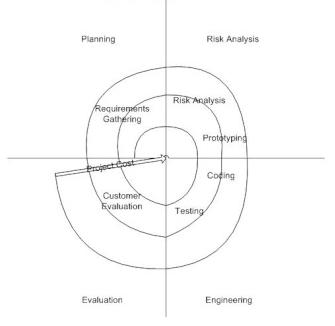
\includegraphics{../../Images/Spiral-model.jpg}
\caption{Spiral model diagram \parencite{spiral}}
\end{figure}

\subsubsection{Time Boxing}\label{time-boxing}

Involves strict deadlines rather than goals. By developing up to the
agreed upon time and evaluating progress this can allow for steadier
development and a set time in mind which provides a deadline for
development.

Evaluating at the end of the time frame can show struggles in the
development process and provides the ability to address them rather than
simply spending more time to complete the goal.

\subsection{Choice of methodology}\label{choice-of-methodology}

After assessing the various forms of project methodologies I have
decided to use an agile methodology most notably the Lean methodology as
this will provide me the ability to develop core functionality in a fast
pace and add other features time permitting. To assist my development I
will also be using time boxing to allocate time for my applications
functions and allow me to perform regular performance reviews so I can
identify time sinks and other issues to allow me to manage them.

\subsection{Project Time line}\label{project-time-line}

Below is a Gantt chart of the overall plan for my project. A Gantt chart
doesn't suit my development methodology very well and so is fairly
high-level overview.

\begin{landscape}
\begin{figure}[htbp]
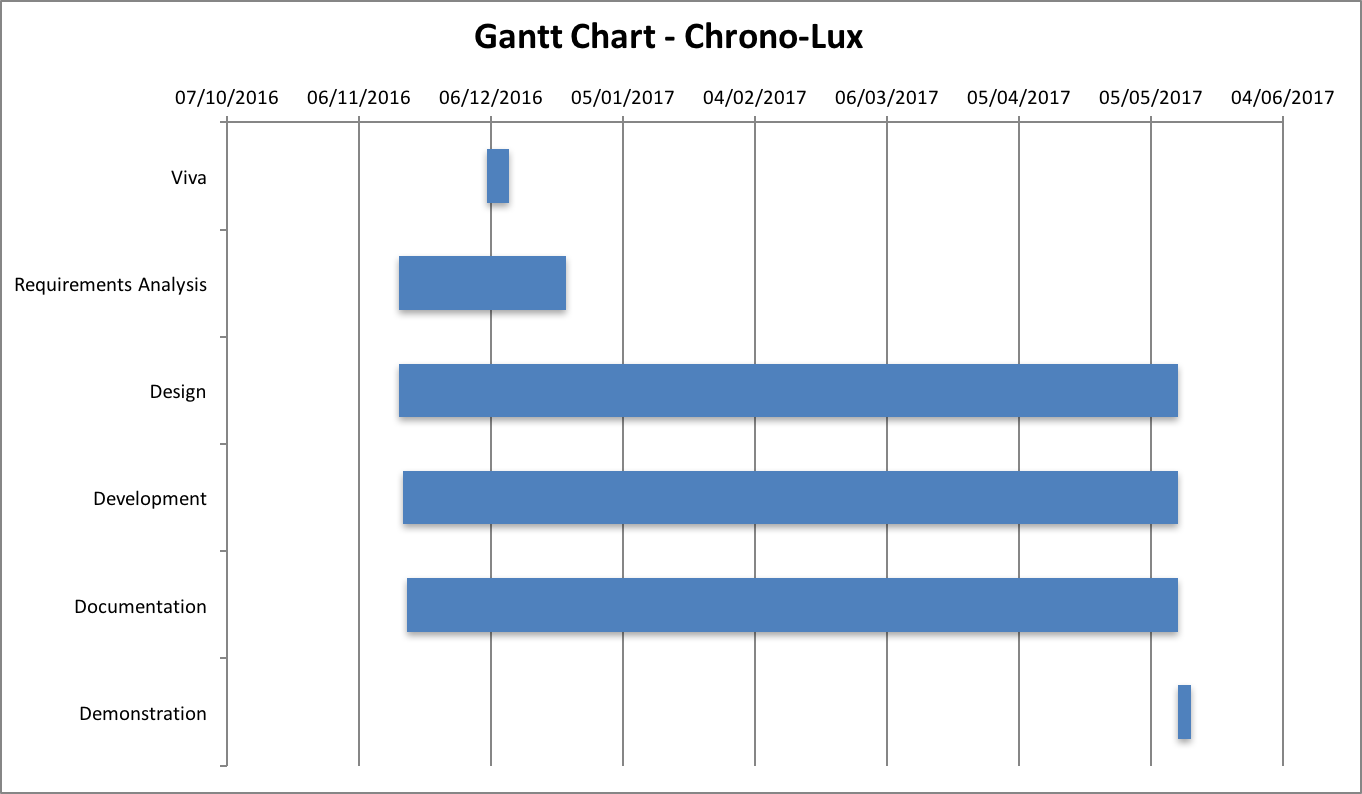
\includegraphics{Images/gantt.png}
\caption{Project Gantt Chart}
\end{figure}
\end{landscape}


\printbibliography
\end{document}
